\section{The Civitas Economica Framework}
\label{sec:method}

Civitas Economica links person-to-person contact, person-to-group influence, and group-to-society market outcomes on a shared clock. Figure~\ref{fig:overview} follows these relations from available observations through valuation and orders to settlement, whose prices and portfolios enter the next step. Let $N$ be the population size, $i,j\in\{1,\dots,N\}$ index agents, and $t\in\{1,\dots,T\}$ index simulation steps. We use the truncation operator $\clip(x,l,u)=\max(l,\min(u,x))$ and the logistic function $\sigma(x)=(1+e^{-x})^{-1}$. Agents allocate cash and shares of one risky asset. Available cash and sellable inventory bound each order.

\begin{figure*}[t]
  \centering
  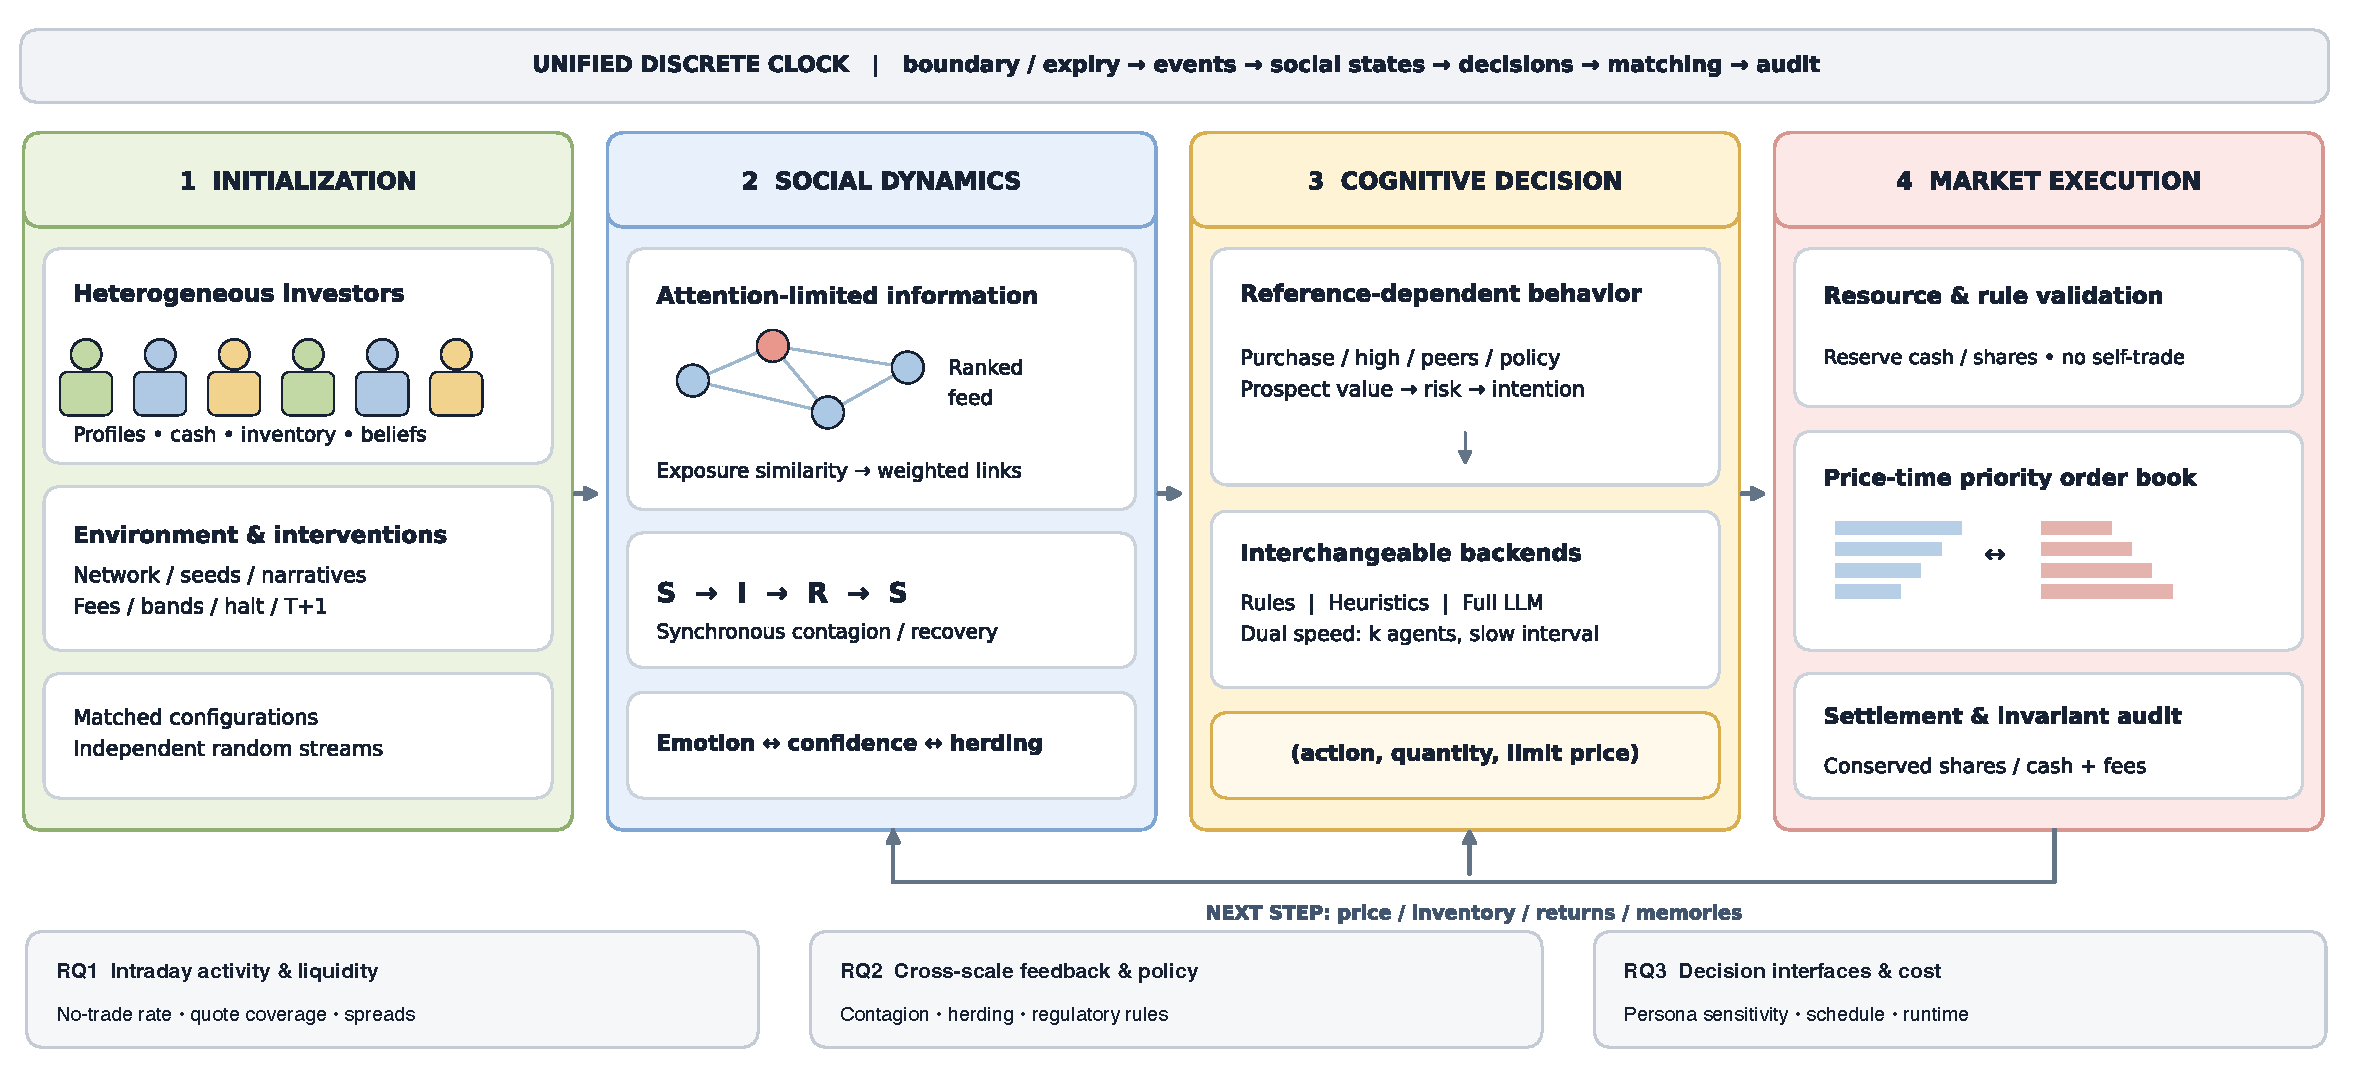
\includegraphics[width=\textwidth]{figures/fig1_methodology_overview.pdf}
  \caption{The Civitas Economica architecture. Portfolio exposures weight ties, group states shape orders, and settlement produces new prices and portfolios. Phases \ref{phase:boundary}--\ref{phase:events} prepare the market. Phases \ref{phase:social}--\ref{phase:behavior} update information and behavior using Equations~\eqref{eq:exposure}--\eqref{eq:confidence_update}. Phase \ref{phase:decision} produces orders through Equations~\eqref{eq:aggregate_v}--\eqref{eq:order_quantity} or the decision interface, which supports the cache in Equation~\eqref{eq:cache_signature}. Phases \ref{phase:execution}--\ref{phase:commit} process arrivals in seeded order, settle trades, and commit the ledger under Equations~\eqref{eq:settle_b}--\eqref{eq:invariants}.}
  \Description{Three economic relation scales linked by an eight-phase clock, from peer exposure and group states to orders, market settlement, and next-step feedback.}
  \label{fig:overview}
\end{figure*}

\subsection{Unified Discrete Clock and Causal Scheduling}
\label{sec:method:clock}

Each step separates updates visible to decision makers from the trades produced by their decisions.
\begin{enumerate}[leftmargin=*, label=(\arabic*), ref=\arabic*]
  \item\label{phase:boundary} \textbf{Trading Day Boundary.} The first day starts at $P_0$. At each subsequent day boundary, where $t>1$ and $(t-1)\bmod T_{\mathrm{day}}=0$, set $P^{\mathrm{base}}_t=P_{t-1}$ and release expired inventory locks. The daily band is $[P_t^{\mathrm{lower}},P_t^{\mathrm{upper}}]=[P^{\mathrm{base}}_t(1-L),P^{\mathrm{base}}_t(1+L)]$.
  \item\label{phase:expiry} \textbf{Order Expiration and Reservation Release.} Cancel expired orders and return remaining reserved cash and shares to available balances.
  \item\label{phase:events} \textbf{Exogenous Events and Public Narratives.} Publish scheduled macroeconomic announcements, earnings reports, or regulatory shocks.
  \item\label{phase:social} \textbf{Social Interaction and Message Filtering.} Update exposure-weighted edges, select messages under the attention budget, and advance the synchronous SIRS process from the post-event states.
  \item\label{phase:behavior} \textbf{Sentiment and Confidence.} Compute herding weights from lagged confidence and the pessimistic-neighbor share. Update sentiment $s_{i,t}$ using post-transition infection, lagged peer sentiment, and the previous return. Update confidence $q_{i,t}$ according to the herding trigger.
  \item\label{phase:decision} \textbf{Cognitive Decisions.} All agents update their reference prices. The activation mask $A^{\mathrm{act}}_{i,t}\sim\mathrm{Bernoulli}(p_{\mathrm{act}})$ is sampled across agents and steps and shared within matched comparisons. Active agents use their assigned backend to return \texttt{(action, quantity, price)}. Inactive agents submit \texttt{HOLD}.
  \item\label{phase:execution} \textbf{Validation, Matching, and Settlement.} Process intents in seeded arrival order, checking cash or sellable shares. Match admissible orders against the book by price and time priority, and settle fills and fees.
  \item\label{phase:commit} \textbf{Ledger Auditing and State Records.} Check cash and share conservation and record execution, ledger, and agent state.
\end{enumerate}

An agent sees the last committed price and book, its current available resources and psychological state, and events visible at the current step. Its own execution receipts become visible from step $t+1$. With a one-step order lifetime, remaining orders expire before new intents arrive, so the quoted depth in the observation is historical.

\subsection{Three Scales and Investor Archetypes}
\label{sec:method:population}

\paragraph{Person to Person.} Exposure similarity determines the weight of a peer relationship. Let $C_{i,t-1}$ and $Q_{i,t-1}$ be the cash and shares held by agent $i$ after step $t-1$. Prices and cash in the behavioral rules are in major currency units. Risk exposure is the fraction of wealth held in the risky asset.
\begin{equation}
x^{\mathrm{exp}}_{i,t-1}=\frac{Q_{i,t-1}P_{t-1}}{C_{i,t-1}+Q_{i,t-1}P_{t-1}+\epsilon}.
  \label{eq:exposure}
\end{equation}
Each edge moves toward a target set by the similarity of the two portfolios.
\begin{equation}
\begin{split}w_{ij,t}=\clip\bigl(&(1-\omega)w_{ij,t-1}\\&+\omega(2-|x_i^{\rm exp}-x_j^{\rm exp}|),w_{\min},w_{\max}\bigr).\end{split}
  \label{eq:edge_weight}
\end{equation}
Both exposures in the edge update are evaluated at step $t-1$. We use $\omega=0.1$ and $(w_{\min},w_{\max})=(1,2)$. Cash and price are expressed in the same currency unit, and $\epsilon>0$ defines exposure for zero wealth. A smaller exposure difference raises the target edge weight. These ties weight neighborhood aggregates. Equation~\eqref{eq:message_score} selects messages under limited attention.

\paragraph{Person to Group.} The selected feed and weighted neighborhood states drive infection, sentiment, and confidence in Equations~\eqref{eq:infection_prob}--\eqref{eq:confidence_update}. The nine archetypes have sampling probabilities of 70\% for retail traders, 8\% for mutual funds, 5\% for pension funds, 4\% for insurers, 4\% for proprietary desks, 4\% for market makers, 1\% for stabilization funds, 2\% for rumor-sensitive traders, and 2\% for arbitrageurs. Archetypes define role labels and the persona-specific decision parameters in Section~\ref{sec:method:cognition}. We sample them independently of the Watts--Strogatz network, so role and network position can vary separately~\cite{watts1998collective}. Baseline loss aversion is $2.25$ for all archetypes.

\paragraph{Group to Society.} This scale represents collective outcomes in the modeled market. Orders from all archetypes meet in the limit order book under common trading rules, producing transaction prices, volume, spreads, and depth. Settlement in Equations~\eqref{eq:settle_b}--\eqref{eq:invariants} changes portfolios. Prices and returns enter the next step's exposure, references, and sentiment. These updates close the feedback from market outcomes to individual decisions.

\subsection{Social Layer: Attention-Bounded Contagion and Confidence-Dependent Herding}
\label{sec:method:social}

\paragraph{Attention-Bounded Information Filtering.} Let $\mathcal N_i$ be agent $i$'s social neighborhood. In phase~(\ref{phase:social}), agent $i$ scores messages from neighbors in the infected state after the external event has been applied.
\begin{equation}
\begin{split}h_{ij,t}={}&\theta_1(1-|s_i-s_j|/2)+\theta_2\ind\{u_i=u_j\}\\&+\theta_3(1-|a_i-a_j|)+\theta_4 Inf_j+\theta_5 E_{ij,t-1}.\end{split}
  \label{eq:message_score}
\end{equation}
The terms measure sentiment similarity, shared topic, risk similarity, source influence, and past exposure. Sentiment and risk come from the previous committed step, and nonnegative weights sum to one. The highest-scoring messages form $\mathcal F_{i,t}$, with at most $A_i$ messages and ties broken by source identifier.

\paragraph{Synchronous SIRS Panic Propagation.} The model represents panic with Susceptible ($S$), Infected ($I$), and Recovered ($R$) states. Infection pressure combines the weighted infection share across the neighborhood with the messages selected by attention.
\begin{equation}
\begin{split}\rho_{i,t}&=\frac{\sum_j w_{ij,t}\ind\{\widetilde X_{j,t}=I\}}{\sum_jw_{ij,t}},\\p^{\rm inf}_{i,t}&=\clip\bigl(\overline{h_{ij,t}\mathrm{sim}_{ij,t}}_{\mathcal F_{i,t}}(\kappa_0+\kappa_1\rho_{i,t})\\&\hspace{5em}+\kappa_2\rho_{i,t},0,1\bigr).\end{split}
  \label{eq:infection_prob}
\end{equation}
Here $\widetilde X$ is the post-event, pre-transition state and $\mathrm{sim}_{ij,t}=1-|s_i-s_j|/2$ uses lagged sentiment. The sums in $\rho_{i,t}$ run over $\mathcal N_i$, and the overbar takes the arithmetic mean of $h_{ij,t}\mathrm{sim}_{ij,t}$ over $\mathcal F_{i,t}$. An empty feed has mean zero, and an isolated agent's infection share is zero. A susceptible agent becomes infected with probability $\clip(\beta p^{\rm inf}_{i,t}c_i,0,1)$, where $c_i$ is herding propensity.

Recovery depends on infection duration and the concentration of an agent's exposure.
\begin{equation}
p^{\rm rec}_{i,t}=\clip\bigl(\gamma(1+\eta_d\widetilde D_{i,t})(1-\eta_e e_{i,t}),0,1\bigr).
  \label{eq:recovery_prob}
\end{equation}
Exposure follows $E_{ij,t}=(1-\zeta_E)E_{ij,t-1}+\zeta_E\ind\{j\in\mathcal F_{i,t}\}$. Its concentration is $e_{i,t}=\sum_j(E_{ij,t}/\sum_kE_{ik,t})^2$, with zero concentration when total exposure is zero. The duration $\widetilde D$ is evaluated before the transition. A recovered agent becomes susceptible with probability $\clip(\delta(1+\eta_\psi p^{\rm inf}_{i,t}),0,1)$. Each transition is sampled from the post-event state. This makes the propagation update synchronous.

\paragraph{Confidence-Dependent Herding.} Continuous sentiment $s_{i,t}\in[-1,1]$ combines inertia, infection, peer sentiment, and the market return.
\begin{equation}
\begin{split}s_{i,t}=\clip\bigl(&(w_i^D-\Delta_{i,t})s_{i,t-1}-w_i^g\ind\{X_{i,t}=I\}\\&+(w_i^N+\Delta_{i,t})\bar s^N_{i,t-1}\\&+w_i^M\clip(r_{t-1}/r_*,-1,1)+\epsilon_s,-1,1\bigr).\end{split}
  \label{eq:sentiment_update}
\end{equation}
The peer term averages lagged sentiment with edge weights. An isolated agent uses its own lagged sentiment. The default return scale is $r_*=0.01$, and $\epsilon_s\sim\mathcal N(0,\sigma_s^2)$ with $\sigma_s=0.02$. Herding transfers weight from the agent's own prior sentiment to that of peers, preserving their combined weight~\cite{deutsch1955study}.
\begin{equation}
\Delta_{i,t}=H_{i,t}\eta_H(1-q_{i,t-1})w_i^D,\qquad H_{i,t}=\ind\{b^N_{i,t}>0.5\}.
  \label{eq:herding_shift}
\end{equation}
Here $b^N_{i,t}$ is the edge-weighted fraction of neighbors with sentiment below $-s_*$. Confidence decreases when the trigger fires and otherwise returns toward $q_0$. The herding ablation sets $\eta_H=\eta_q=0$ and retains the recovery term.
\begin{equation}
\begin{split}q_{i,t}=\clip\bigl(&q_{i,t-1}-H_{i,t}\eta_q(1-q_{i,t-1})\\&+(1-H_{i,t})\eta_{\rm rec}(q_0-q_{i,t-1}),0,1\bigr).\end{split}
  \label{eq:confidence_update}
\end{equation}


\subsection{Behavioral Core: Multi-Reference Prospect Theory and Order Generation}
\label{sec:method:behavior}

\paragraph{Four Adaptive Reference Prices.} After the social update, agents update four anchors in phase~(\ref{phase:decision}) for acquisition cost ($R^p$), the rolling local high ($R^h$), peer consensus ($R^n$), and the policy signal ($R^e$).
\begin{align}
 R^p_{i,t}&=(1-\kappa_p)R^p_{i,t-1}+\kappa_p T^p_{i,t},\label{eq:ref_p}\\
 R^h_{i,t}&=(1-\kappa_h)R^h_{i,t-1}+\kappa_h \max_{v=\max(0,t-H_h)}^{t-1}P_v,\label{eq:ref_h}\\
 R^n_{i,t}&=(1-\kappa_n)R^n_{i,t-1}+\kappa_nP_{t-1}(1+\xi_n\bar s^N_{i,t-1}),\label{eq:ref_n}\\
 R^e_{i,t}&=(1-\kappa_e)R^e_{i,t-1}+\kappa_eP_{t-1}(1+\xi_e u_t^{\rm policy}).\label{eq:ref_e}
\end{align}
For a nonempty position the cost target is $T^p=K$, where $K$ is the position cost basis excluding fees. An empty position uses $T^p=P_{t-1}$. A policy state persists until a subsequent event changes it. Event text is visible at release.

\paragraph{Prospect Valuation and Loss Pressure.} An asymmetric power function maps reference deviations to prospect value~\cite{tversky1992advances}.
\begin{equation}
v_i(z)=\begin{cases}z^\alpha&z\ge0,\\-\lambda_i(-z)^\alpha&z<0.\end{cases}
  \label{eq:prospect_v}
\end{equation}
In the full model, $\lambda_i>1$ sets loss aversion and $\alpha\in(0,1)$ sets diminishing sensitivity. We define signed deviations from the cost and price high using the reference as the denominator. For peer and policy anchors we use the latest price as denominator and reverse the sign convention. The weighted sum enters the value function once.
\begin{equation}
\begin{split}x^\bullet_{i,t}&=\begin{cases}(P_{t-1}-R^\bullet_{i,t})/R^\bullet_{i,t}&\bullet=p,h,\\(R^\bullet_{i,t}-P_{t-1})/P_{t-1}&\bullet=n,e,\end{cases}\\z_{i,t}&=\sum_\bullet\omega_\bullet x^\bullet_{i,t},\quad V_{i,t}=v_i(z_{i,t}),\quad d_{i,t}=\tanh(\kappa_vV_{i,t}).\end{split}
  \label{eq:aggregate_v}
\end{equation}
The retrospective loss fraction $b_{i,t}=(\omega_p\mathbf{1}\{P_{t-1}<R^p_{i,t}\}+\omega_h\mathbf{1}\{P_{t-1}<R^h_{i,t}\})/(\omega_p+\omega_h)$ weights the cost and high-price references above the current price and enters the bounded loss-pressure function.
\begin{equation}
  \ell_{i,t} = \clip\left( \lambda_i (1 + \chi b_{i,t}), \ell_{\min}, \ell_{\max} \right).
  \label{eq:loss_pressure}
\end{equation}
Current risk tolerance $a_{i,t}\in[0,1]$ combines confidence, lagged risk tolerance, sentiment, valuation direction, and loss pressure.
\begin{equation}
\begin{split}a_{i,t}=\clip\bigl(&\omega_a^q q_{i,t}+\omega_a^a a_{i,t-1}+\omega_a^s s_{i,t}\\&+\omega_a^d d_{i,t}-\omega_a^\ell\max(0,(\ell_{i,t}-1)/\nu),0,1\bigr).\end{split}
  \label{eq:risk_tolerance}
\end{equation}

\paragraph{Trading Intention and Limit Orders.} Valuation direction, sentiment, and risk tolerance determine the intention score $\tau_{i,t}\in[-1,1]$.
\begin{equation}
\tau_{i,t}=\clip\bigl(\omega_\tau^d d_{i,t}+\omega_\tau^s s_{i,t}+\omega_\tau^a(a_{i,t}-0.5),-1,1\bigr).
  \label{eq:intent_score}
\end{equation}
At threshold $\delta_a\ge0$, the agent draws a buy, sell, or hold action using the following probabilities.
\begin{equation}
\begin{split}p_i^b&=\sigma(\kappa_a(\tau_{i,t}-\delta_a)),\\p_i^s&=\sigma(-\kappa_a(\tau_{i,t}+\delta_a)),\qquad p_i^h=1-p_i^b-p_i^s.\end{split}
  \label{eq:action_selection}
\end{equation}
An independent $U_i\sim U(0,1)$ scales the order size. The buy fraction is $f_i^b=U_i[f_{\min}+(f_{\max}-f_{\min})a_i]$. The sell fraction is $f_i^s=U_i[f_{\min}+(f_{\max}-f_{\min})\max(-\tau_i,0)]$. Rule baselines share the mean-corrected lognormal quote perturbations, drawn independently of action direction.
\begin{equation}
\begin{split}\widetilde p_i&=P_{t-1}\exp(\epsilon_p-\sigma_p^2/2),\\p_i^{\rm lim}&=\Delta_p\max\{1,\operatorname{round}_{\rm even}(\widetilde p_i/\Delta_p)\}.\end{split}
  \label{eq:limit_price}
\end{equation}
Here $\epsilon_p\sim\mathcal N(0,\sigma_p^2)$. At a rounding tie, the quote rounds to an even tick. The exchange rejects orders outside the daily price band. Quantities are integers bounded by available resources.
\begin{equation}
  n_i = \begin{cases}
    \bigl\lfloor f^b_{i,t} C_{i,t}^{\mathrm{free}} / \bigl(p_i^{\mathrm{lim}}(1+c)\bigr) \bigr\rfloor & \mathrm{BUY}, \\
    \bigl\lfloor f^s_{i,t} Q_{i,t}^{\mathrm{free}} \bigr\rfloor & \mathrm{SELL}.
  \end{cases}
  \label{eq:order_quantity}
\end{equation}
Here $c$ is the commission rate. Zero quantities become \texttt{HOLD}.

\subsection{Microstructure, Limit Order Book, and Ledger Invariants}
\label{sec:method:microstructure}

\paragraph{Escrow Reservation and Price--Time Priority.} Buy orders reserve cash for limit-price notional and buyer commission. Sell orders reserve sellable shares. The ledger tracks these reservations within each account. The ledger stores $10^6$ integer micro-units per major currency unit: $C_{i,t}^{\rm minor}=10^6 C_{i,t}$. Fill notionals and fees use the same micro-unit scale. For integer fill notional $V$, each side pays commission $f_c=\lfloor cV\rfloor$ and the seller pays tax $f_\tau=\lfloor\tau^{\rm tax}V\rfloor$.

Bids are ordered by descending price and asks by ascending price, with earlier orders first at each price. Crossing orders match at the resting price. A fill of $q^*$ shares updates the buyer $b$, seller $s$, and the fee account $F^{\rm minor}$ as follows.
\begin{align}
  C_b^{\rm minor} &\gets C_b^{\rm minor} - V-f_c, \quad Q_b \gets Q_b + q^*, \label{eq:settle_b} \\
  C_s^{\rm minor} &\gets C_s^{\rm minor} + V-f_c-f_\tau, \quad Q_s \gets Q_s - q^*, \label{eq:settle_s} \\
  F^{\rm minor} &\gets F^{\rm minor} +2f_c+f_\tau. \label{eq:settle_fees}
\end{align}
A fill releases excess escrow for the executed quantity. Resources for any unfilled quantity remain reserved until execution, cancellation, or expiration.

\paragraph{Ledger Conservation.} Reserved resources remain part of account balances. At every commit, the engine audits total cash across the agent and fee accounts and total shares across agents.
\begin{equation}
\begin{aligned}
 \sum_i C_{i,t}^{\rm minor}+F_t^{\rm minor}&=\sum_i C_{i,0}^{\rm minor}+F_0^{\rm minor},\\
 \sum_{i=1}^N Q_{i,t}&=\sum_{i=1}^N Q_{i,0}.
\end{aligned}
  \label{eq:invariants}
\end{equation}
Any nonzero residual triggers an audit error.

\subsection{Cognitive Architectures and Dual-Speed Scheduling}
\label{sec:method:cognition}

All four backends share information eligibility and return \texttt{(action, quantity, price)}. The same execution kernel validates and matches their orders.
\begin{enumerate}[leftmargin=*, label=(\arabic*)]
  \item \textbf{Numerical Rules (System 1).} Evaluate Equations~(\ref{eq:exposure})--(\ref{eq:order_quantity}) as the rule baseline.
  \item \textbf{Persona Heuristics.} Adjust a target portfolio exposure for valuation, trend, and sentiment. An archetype-specific band and a resource cap govern the resulting order.
  \item \textbf{Full LLM Agents (System 2).} Serialize the agent's profile, account state, market facts, and eligible records. Validate response identity and intent type, and check that \texttt{evidence\_ids} are unique members of the visible ID set (Appendix~\ref{app:prompt}). The exchange checks price bands and available resources at execution.
  \item \textbf{Dual-Speed Hybrid Scheduling.} All agents perform lightweight System 1 updates. A fixed set of $k$ agents sampled by persona requests System 2 responses when active and $t\bmod T_{\mathrm{slow}}=0$.
\end{enumerate}

The market runner admits rule decisions and both synthetic and archived model responses. Live model requests use the same decision contract in a separate fixed-observation harness.

\paragraph{Resource-Aware Strategy Caching.} At a System 2 request step, the scheduler caches a normalized direction and resource commitment so later orders can adapt to current prices and balances.
\begin{equation}
\begin{aligned}
 \widehat d_i &=
 \begin{cases}
   +1 & \mathrm{BUY}, \\
   -1 & \mathrm{SELL}, \\
   0 & \mathrm{HOLD},
 \end{cases} \\
 \widehat f_i &=
 \begin{cases}
   \min\!\bigl(1,n_i/M_i^{\mathrm{action}}\bigr) & M_i^{\mathrm{action}}>0, \\
   0 & \text{otherwise.}
 \end{cases}
\end{aligned}
  \label{eq:cache_signature}
\end{equation}
Here $M_i^{\mathrm{action}}$ is conservative capacity at the requested limit price under a continuous commission budget bound. A \texttt{HOLD} decision has zero resource commitment. When reusing the cache, an active agent keeps $\widehat d_i$ and $\widehat f_i$, recomputes a limit price around $P_{t'-1}$ with the shared quote perturbation, and floors the committed fraction of current capacity to obtain an integer quantity. Reuse is allowed for ages $1$ through $A_{\max}$, inclusive. A missing or expired entry invokes the rule policy. A recognized response failure clears the cache and returns \texttt{HOLD}. A reused intent with zero final quantity returns \texttt{HOLD}.

\paragraph{Scheduled Model Request Budget.} Over $T$ steps, full LLM scheduling offers $p_{\mathrm{act}}NT$ expected request opportunities and dual-speed scheduling offers $p_{\mathrm{act}}k\lfloor T/T_{\mathrm{slow}}\rfloor$. Their ratio is approximately
\begin{equation}
  \text{Request ratio} \approx \frac{k}{N \cdot T_{\mathrm{slow}}}.
  \label{eq:cost_ratio}
\end{equation}
For $N=100$, $k=10$, and $T_{\rm slow}=10$, a horizon divisible by $T_{\rm slow}$ yields 99\% fewer expected request opportunities. Actual cost also depends on response usage and execution time.
\paragraph{Analysis Tools.} We used OpenAI Codex to assist with implementation cross-checks, analysis of archived records, and manuscript editing. We checked the reported values against the archived data.
